\chapter{Test}\label{Test}

\section{Connection test}\label{test:Connect}
\begin{figure}[H]
    \centering
    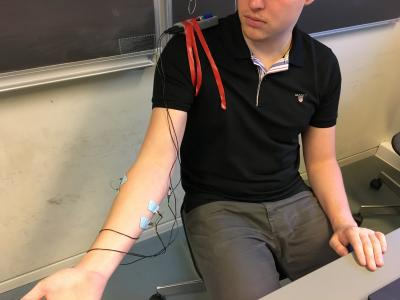
\includegraphics[width=10cm,height=5cm]{Figures/Technical_figures/image0.jpg}
    \caption{Electrodes and greybox is mounted on the test person}
    \label{fig:connectiontest}
\end{figure}

\subsection*{Layout}
Six electrodes providing the data fro the EMG was places on a test person. The measuring box should then be able to pick up the EMG of the muscles, along with accelerometer data from the IMU. The goal of this test is to see if the received data from the measuring box is transferred correctly into the Teensy micro controller, and further more onto the robot. The electrodes are place so neutral is on the elbow and two muscles are selected in a way that if the test person moves the arm one way the robot go forward and the other way backwards. These muscles can be found by instructing the test person to move the hand to the point of maximum extensions and search for the muscles that is most contracted on the upper part of the lower elbow.

\subsection*{Success criteria}
 The robot must then be able to receive and act upon the signals from the measuring box. By switching the active joint on the robot using the IMU and turning in both directions using the EMG signal.
\subsection*{Iterations}
\begin{enumerate}
    \item The connection was successful in the first test.
\end{enumerate}
\subsection*{Result}
 It was possible to connect to the Teensy simply by turning on the measuring box, the wireless connection between the Teensy and the measuring box is then complete which insures the users safety. It was clear that data was transferred correctly since it was possible to move the directions of choice and change the joint to move about.\\
\newpage
\section*{EMG Thresholds}
\begin{figure}[H]
    \centering
    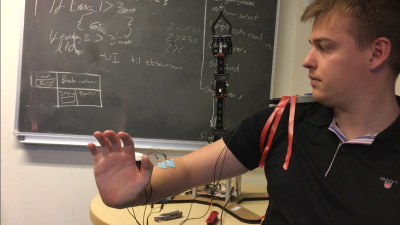
\includegraphics[width=10cm,height=5cm]{Figures/Technical_figures/image2.png}
    \caption{The user sits in a contracted posistion for 3 minutes}
    \label{fig:connectiontest}
\end{figure}
\subsection*{Layout}
This test is done with the same layout as in Section \ref{test:Connect}. The goal of this test is to fine tune the Thresholds activating the robot, in such a way that the user does not get exhausted from using the arm, and in a way that the noise wont be taken into the threshold.\\
This test complies with the code \ref{fig:AngleSel}.\\
Furthermore a video is taken to calculate the latency from  when the movement of the test person is given to the manipulator responds which complies with requirement: \ref{test:Latency}.
\subsection*{Success criteria}
 If the robot is able to  move reliably in both directions without tiring the test person the test is an success. This means that the test person must be able to hold the pose for 3 min, without being exhausted. and the robot must then be able to use that signal reliably and within 1 second.
\subsection*{Iterations}
\begin{enumerate}
    \item In the first test the contraction was set to 800 both in EMG1 and in EMG2, which resulted in failure to keep the muscle contracted in 3 minutes.
    \item The second test the contraction was set to 500, which resulted in a slightly sore muscle after 3 minutes.
    \item Test 3 was a success due to the test person could easily manoeuvre the robot without sore muscles and noise interference. 
    \item Test 4 included a video of the test person, which is used to calculate the time it takes for a contraction to be uploaded to the manipulator.
\end{enumerate}
\subsection*{Result}
Contraction niveau has been set to 300, which results in no sore muscles and no noise interference. While the manipulator moved reliably and only moved when the test person wanted to move it. This complies with requirement R\ref{test:EMG}.\\
The video resulted in 
\newpage
\section{Lift Test} \label{sec:Lift}
\begin{multicols}{2}
\begin{figure}[H]
    \centering
    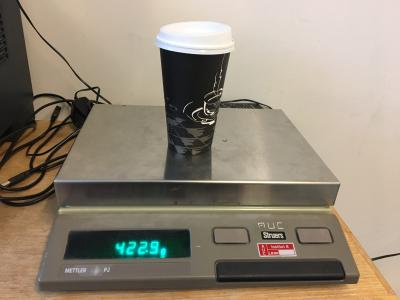
\includegraphics[width=0.45\textwidth, height=5cm]{Figures/Technical_figures/image3.jpg}
    \caption{A cup of tea weighing 422.9g}
    \label{fig:Tea}
\end{figure}
\columnbreak
\begin{figure}[H]
    \centering
    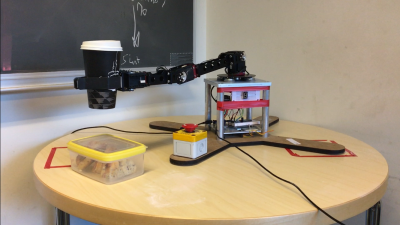
\includegraphics[width=0.45\textwidth,height=5cm]{Figures/Technical_figures/image4.png}
    \caption{The manipulator holds the cup in a streched out posistion.}
    \label{fig:stretch}
\end{figure}
\end{multicols}

\subsection*{Layout}
The sEMG electrodes will be attached as in \ref{test:Connect} and used to control the manipulator.
The manipulator will be moved to a streached position as seen in figure \ref{fig:stretch} and the the weighted cup will be placed in the end effector as seen in figure \ref{fig:Tea}. 
\subsection*{Success criteria}
To succeed the manipulator needs to lift an object with a mass of $500g$
\subsection*{Iterations}
\begin{enumerate}
    \item The first test was done with a 523g bottle, this was to measure if it could lift over $500g$, but it failed.
    \item Test nr.2 was done with a cup of $500g$, which failed. 
    \item The previous tests failed, so it was decided to use a cup of 422.9g and test the PWM signal instead. The PWM signal is set to 200 at the start of this test. First the robot was not able to lift the cup, therefore, the PWM signal is set to 250.
    \item This was still not enough, so the PWM is set to 300. 
    \item Same as in iteration 2, and the PWM is set to 350.
    \item A PWM of 350 is almost enough.
    \item PWM was set to 360, the robot could now move the elbow joint to lift the cup.
\end{enumerate}
\subsection*{Result}
The manipulator succeeded in raising the cup of tea, which measured 422.5g. The requirement of lifting $500g$ is not met, however, the result is satisfactory. Furthermore the PWM threshold was decided and calibrated.\\
This test complies with requirement R\ref{req:extension}
\newpage
\section{Test of the forces on the robot}
\begin{figure}[H]
    \centering
    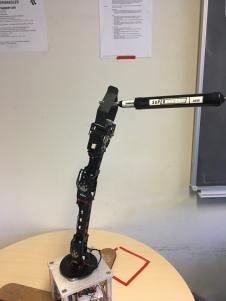
\includegraphics[width=7cm,height=7cm]{Figures/Technical_figures/image5.jpg}
    \caption{The manipulator is pulled with a newton-meter to calculate the force in N}
    \label{fig:Nm}
\end{figure}
\subsection*{Layout}
The manipulator is pre-set to angles and PWM, which is 2000 for all the angles and 360 for the PWM. A newton-meter was used to measure all the forces on the joints, as seen in figure \ref{fig:Nm}.\\

\subsection*{Success criteria}
We want the forces on all of the joints to be below 194.50N
\subsection*{Iterations}
\begin{enumerate}
    \item The first test decided how much force it was required to seperate the fingers, which was 20N.
    \item The second test decided how much force it would take to rotate around the shoulder joint.
    The result was 14N
    \item The third test decided how much force it would take to rotate around the shoulder elbow joint. The result was 21N
    \item The fourth test decided how much force it would take to rotate around the shoulder base joint. The result was 14N
    \end{enumerate}
\subsection*{Result}
Each separate joint is below the required N, which complies with requirement R\ref{req:force}.
\newpage
\section{IMU test}
\subsection*{Layout}
This test is done with the same layout as in Section \ref{test:Connect}. The goal of this test is to fine tune the motor select function in the system. 
\subsection*{Success criteria}
 If the robot is able to  move reliably switch the joint that is active based on the data from the IMU. This means that the user must be able to get to the right join tin both directions 10 times.
\subsection*{Iterations}
\begin{enumerate}
    \item {\textbf{Starting values:} \textit{Accelerator threshold = 700 \& 300 }}
\end{enumerate}
\subsection*{Result}
\newpage


\section{Final Test}

\begin{figure}[H]
    \centering
    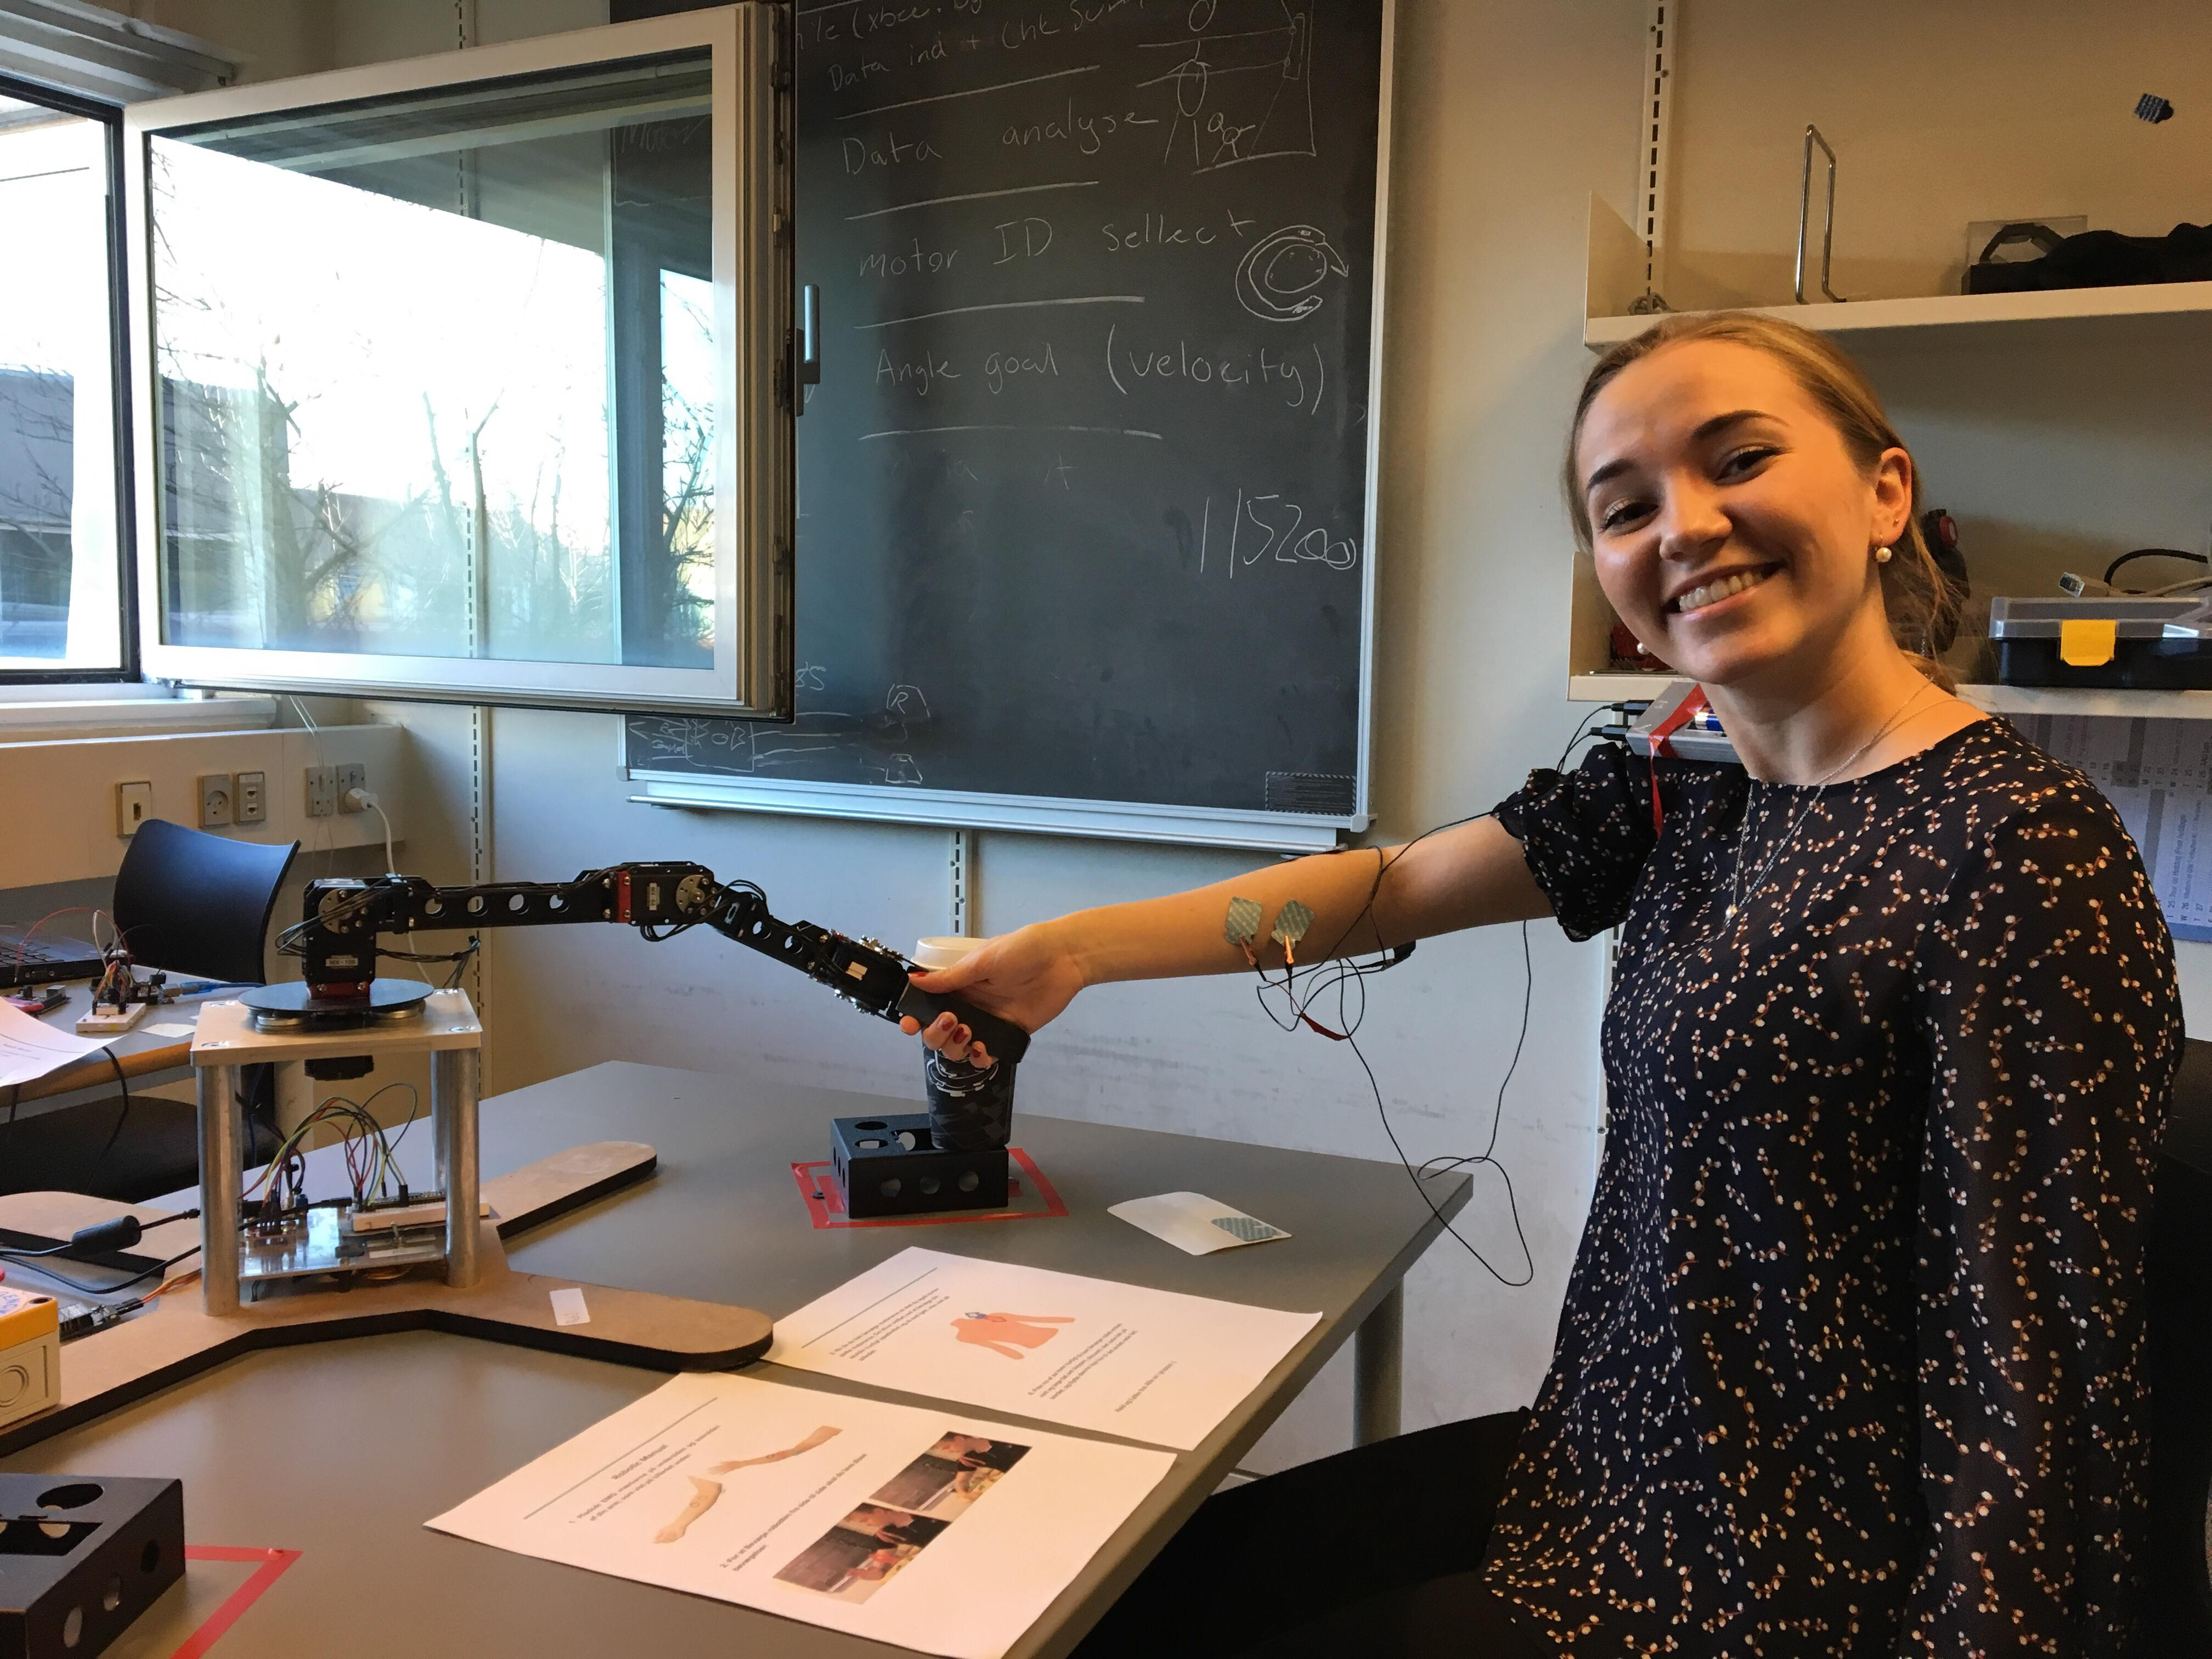
\includegraphics[width=7cm,height=7cm]{Figures/Technical_figures/anna.jpg}
    \caption{Anna Julie Qvist testing the robot}
    \label{fig:Anna}
\end{figure}

\subsection*{Layout}
This test is done with the same layout as in Section \ref{test:Connect}. This time the manipulator is controlled by several people from outside the group to test if its intuitive to use.
\subsection*{Success criteria}
 The test person have to use the manipulator to move a cup of tea like in test \ref{sec:Lift}, in under 3 minutes. A exercise round is given to the test person so the person can get used to the contractions and accelerations. In the second test they have to do their best to move the cup under 3 minutes.
\subsection*{Iterations}
\begin{enumerate}
    \item Anna Julie Qvist managed to use the manipulator and move the cup of tea in 3.46 minutes. There was some minor disruptances 
    \item Ole Managed to use the manipulator and move the cup of tea in 1.13 minutes.
\end{enumerate}
\subsection*{Result}


